% !TEX TS-program = pdflatexmk
\documentclass[12pt]{amsart}

%\usepackage[parfill]{parskip}    % Activate to begin paragraphs with an empty line rather than an indent

\usepackage[margin=1in]{geometry}

\usepackage{amsmath,amssymb,amsthm,latexsym,graphicx}
\usepackage{setspace} %used for doublespacing, etc.
\usepackage{hyperref}
\usepackage[dvipsnames,usenames]{color}
\usepackage[all]{xy}
\usepackage{fancyhdr}
\pagestyle{fancy}
	\renewcommand{\headrulewidth}{0.5pt} % and the line
	\headsep=1cm

\DeclareGraphicsRule{.tif}{png}{.png}{`convert #1 `dirname #1`/`basename #1 .tif`.png}

%Some useful environments.
\newtheorem*{theorem}{Theorem}
\newtheorem*{corollary}{Corollary}
\newtheorem*{conjecture}{Conjecture}
\newtheorem*{lemma}{Lemma}
\newtheorem*{proposition}{Proposition}
\newtheorem*{definition}{Definition}
\newtheorem*{example}{Example}
\newtheorem*{axiom}{Axiom}
\theoremstyle{remark}
\newtheorem*{remark}{Remark}
\newtheorem*{observation}{Observation}
\newtheorem*{basic notion}{Basic Notion}
\newtheorem*{fact}{Fact}
\newtheorem*{exercise}{Exercise}%[section]

%For GeoGebra
\usepackage{pgf,tikz,pgfplots}
\pgfplotsset{compat=1.15}
\usepackage{mathrsfs}
\usetikzlibrary{arrows, angles, quotes}
\newcommand{\degre}{\ensuremath{^\circ}}
\tikzstyle{point}=[circle, fill, inner sep=0pt, minimum size=4pt]


%Some useful shortcuts for our favorite sets of numbers
%Note, you can use these WITHOUT entering math mode

\newcommand{\RR}{\ensuremath{\mathbb R}}
\newcommand{\NN}{\ensuremath{\mathbb N}}
\newcommand{\ZZ}{\ensuremath{\mathbb Z}}
\newcommand{\QQ}{{\ensuremath\mathbb Q}}
\newcommand{\CC}{\ensuremath{\mathbb C}}
\newcommand{\EE}{{\ensuremath\mathbb E}}

%Some useful shortcuts for formatting lists
\newcommand{\bc}{\begin{center}}
\newcommand{\ec}{\end{center}}
\newcommand{\be}{\begin{enumerate}}
\newcommand{\ee}{\end{enumerate}}
\newcommand{\bi}{\begin{itemize}}
\newcommand{\ei}{\end{itemize}}

%Some useful shortcuts for formatting mathematical symbols
\newcommand{\ol}[1]{\overline{#1}}
\newcommand{\oimp}[1]{\overset{#1}{\iff}} %labeled iff symbol
\newcommand{\bv}[1]{\ensuremath{ \vec{\mathbf{#1}}} } %makes a vector.
\newcommand{\mc}[1]{\ensuremath{\mathcal{#1}}} %put something in caligraphic font
\newcommand{\bsl}[1]{\texttt{\symbol{92}{\em #1}}} %for backslashes.
\newcommand{\normale}{\trianglelefteq}
\newcommand{\normal}{\triangleleft}

\chead{MATH F305: Geometry Summary Sheet}
\pagestyle{fancy}


\begin{document}

\thispagestyle{fancy}
\section{Collected Observations, Basic Notions and Facts}
\subsection{Absolute Geometry}
\begin{axiom} A straight line segment can be drawn between any two distinct points.\end{axiom}
\begin{axiom} A straight line segment may be extended to a line.\end{axiom}
\begin{axiom} Given a line segment a circle may be drawn with the segment as radius and one end point at the center.\end{axiom}
\begin{axiom} All right angles are congruent.\end{axiom}

\subsection{Observations}
\begin{observation} Sets of parallel lines converge to a point in an image when they are not parallel to the picture plane. Lines parallel to the picture plane remain parallel.
\end{observation}
\begin{basic notion} We have two projection models, the artist and screen, and the camera obscura.\end{basic notion}
\begin{fact} Parallel lines may be understood as having the same direction vector, as being equidistant from each other at all points, or as not meeting (in 2D).\end{fact}
\begin{observation} We know of three kinds of perspective drawings of a box... One point, two point, and three point. They are determined by the number of vanishing points the edges of the box have. \end{observation}
\begin{definition} A \emph{pencil of lines} is a collection of lines that either all pass through the same point or all are parallel to the same line.
\end{definition}

We should remember the methods discussed in class for constructing boxes or letters using mathematical perspective methods. Anyone willing to write up their favorite way of completing the letter T?

\begin{observation} The possible images of a point are the empty set, a point, a line and a plane.

The possible images of a line are a point, a line and a line with one missing point.

The possible images of a plane are \ldots
\end{observation}
\begin{observation} When thinking about the images of geometric objects it is important to DRAW the lines connecting the objects THROUGH the observation point TO the image plane. It is also important to be GENERIC in placing our objects (unless there is good reason not to).\end{observation}
\begin{fact} Top and side views are \emph{parallel} projections onto a plane. They are not projections \emph{through a point}.\end{fact}
\begin{definition} A \emph{point} is any element of the set space without any dimensional attribute like length, area, volume, \ldots
\end{definition}
\begin{definition} A \emph{line segment} is the shortest path between two points.
\end{definition}
\begin{definition} A \emph{ray} is the shortest path between two points and its infinite extension to one of its two ends.
\end{definition}
\begin{definition} A \emph{line} is the shortest connection between two points and its infinite extension to both sides.
\end{definition}

\section{Collected Results}
\subsection{Euclidean geometry axioms}
\begin{description}
\item[Two points determine a line] A straight line segment can be drawn between two points.
\item[Line extension] A straight line segment may be extended to a line.
\item[Line segment determines a circle] Given a line segment a circle may be drawn with the segment as radius, and one endpoint at the center.
\item[Right angle congruence] All right angles are congruent.
\item[Playfair's Axiom] Given a line and a point in a plane, the point not incident with the line, there exists a unique line in the plane that is incident with the point but not incident with the line. That is, there is a uinique line in the plane that is parallel to the first line and that passes through the point.
\item[Measurement] Define an arbitrary line segment or angle to have unit length or unit angle measurement of 1. Then every other line segment or any other angle has a measurement relative to this unit measurement.
\item[Sum of Lengths] If $A, B, C$ are in that order along a line, then the sum of the directed distance from $A$ to $B$ and the directed distance from $B$ to $C$ equals the directed distance from  $A$ to $C$. In similarity the same thing applies to angles.
\item[Line Segment Copy] If  a line segment is defined through $A$ and $B$ and $A'$ is a point on a line $l$, then upon a given side of $A'$ on $l$, there is only one point $B'$ such that the line segment given through $A$ and $B$ is congruent to the line segment given by $A'$ and $B'$. In similarity the same thing applies to angles.
\item[Transitivity of Congruence] If line segment one and two are congruent are congruent and line segment two and three are congruent, then line segment one and three are congruent. In similarity the same thing applies to angles.
\item[SAS] For two triangles, if two corresponding sides and the angle between them are congruent, then the triangles are congruent.
\item[SSS] For two triangles, if all three corresponding sides are congruent, then the triangles are congruent.
\end{description}

\subsection{Some Euclidean Geometry Theorems}
\begin{description}
	\item[Sum of Interior Angles] is two right angles.
	\item[Vertical Opposite Angles] If a line is cut by a transversal, then the vertical angles are congruent.
	\item[Alternate Interior Angles] If a pair of lines is cut by a transversal, then the alternate interior angles are congruent.
	\item[Corresponding Angles - $\square$ 4.1.2] If a pair of parallel lines is cut by a transversal, the corresponding angles are congruent.
	\item[Triangle Angle Sum] The sum of the interior angles of a triangle is a straight angle.
	\item[ASA] For two triangles, if two corresponding angles and the side between them are congruent, then the triangles are congruent.
	\item[SAA] For two triangles, if two corresponding angles and one of the sides not between them are congruent, then the triangles are congruent.
	\item[SAS similarity] If $\triangle ABC$ and $\triangle DEF$ such that $\angle ABC\cong\angle DEF$ and $\frac{||AB||}{||DE||}=\frac{||BC||}{||EF||}$ then $\triangle ABC\sim\triangle DEF$.
	\item[AAA$\iff\sim\triangle$]
\end{description}
\smallskip

\begin{proposition}[$\bigcirc$ 1.1] Suppose we have a viewpoint $A$, a picture plane $\omega$, and a line segment $\ol{AB}$ parallel to the picture plane of length $L$. Then if $d$ is the distance between $A$ and $\omega$, and $D$ the distance between $A$ and the plane containing $AB$, the length of the image $l$ in $\omega$ is $l=\frac{Ld}{D}$.
\end{proposition}
\smallskip

\begin{proposition}[$\square$ 2.1] The intersection of two pencils of lines as defined in \S 2 is at most one line.
\end{proposition}
\smallskip

\begin{theorem}[Ceva] Let $\triangle ABC$ be a triangle, and let $D,E$ and $F$ be on the lines $BC, CA$ and $AB$ respectively such that lines $AD, BE$ and $FD$ are concurrent. Then $$\frac{|AF|}{|FB|}\cdot\frac{|BD|}{|DC|}\cdot\frac{|CE|}{|EA|}=1.$$
\end{theorem}
\smallskip

\begin{theorem}[Converse  of Ceva's Theorem] Let $\triangle ABC$ be a triangle,
	and let $D, E,$ and $F$ be on the lines $BC, CA,$ and $AB$ respectively. If

	\begin{equation*}
		\frac{|AF|}{|FB|} \cdot \frac{|BD|}{|DC|} \cdot \frac{|CE|}{|EA|} = 1
	\end{equation*}

then the lines $AD, BE,$ and $FC$ are concurrent.
\end{theorem}
\smallskip

\begin{theorem}[Menelaus] Let $\triangle ABC$ be a triangle, and let a transversal line intersect sides $BC, CA$ and $AB$ at $D, E$ and $J$ respectively such that $D, E$ and $J$ are distinct from $A, B$ and $C$. Then $$\frac{|AJ|}{|JB|}\cdot\frac{|BD|}{|DC|}\cdot\frac{|CE|}{|EA|}=-1.$$
\end{theorem}
\smallskip

\begin{definition} Let $\triangle ABC$ be a triangle, and let a transversal line
	intersect sides $BC, CA,$ and $AB$ at $D, E,$ and $J$ respectively such that
	$D, E,$ and $J$ are distinct from $A, B,$ and $C$. Denote the intersection
	points by $X = AD \cdot BE$ and $F = CX \cdot AB$. Then we say the points
	$AFBJ$ form a harmonic set (which we denote by $H(AB, FJ)$).

\end{definition}
\smallskip

\begin{theorem}[Harmonic Ratio] Let $A, F, B$, and $J$ be four points along a line, in that order. This set of points is a harmonic set if and only if $$\frac{|AF|}{|FB|}\cdot\frac{|BJ|}{|JA|}=-1.$$
\end{theorem}
\smallskip

\begin{lemma}[Star Trek] Let $O$ be the center of a circle, and $P, Q$ and $R$
	be points on the boundary of the circle. Then $\angle QOR = 2 \cdot \angle QPR$.

	\begin{center}
		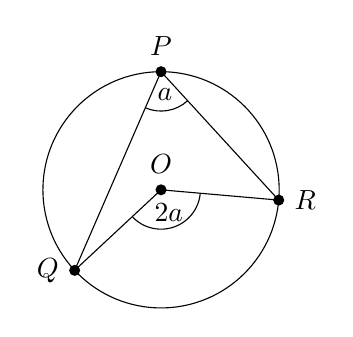
\begin{tikzpicture}[scale=1.5]
			\coordinate (O) at (0,0);
			\coordinate (P) at (90:1);
			\coordinate (Q) at (223:1);
			\coordinate (R) at (355:1);

			\node[point] at (O)[label=above:$O$] {};
			\node[point] at (P)[label=above:$P$] {};
			\node[point] at (Q)[label=left:$Q$] {};
			\node[point] at (R)[label=right:$R$] {};

			\pic [draw, "$2a$", angle eccentricity=0.6] {angle = Q--O--R};
			\pic [draw, "$a$", angle eccentricity=0.6] {angle = Q--P--R};

			\draw (Q)--(P)--(R)--(O)--cycle;

			\draw (O) circle (1);
		\end{tikzpicture}
	\end{center}
\end{lemma}
\smallskip

\begin{theorem}[Thale] If $A$ is a point on a circle and $B,C$ are the end points of a diameter, then the angle $\angle BAC$ is  a right angle.
\end{theorem}
\smallskip

\begin{lemma}[Carpenter's Lemma] A point $P$ forms a right angle $\angle APB$ with a line segment $\ol{AB}$ iff $P$ is a point on the circle with $\ol{AB}$ as its diameter (other than $A$ or $B$).\end{lemma}
\smallskip

\section{Extended Euclidean Space}

\begin{definition} 
For a line $\ell \subset \RR^2$, the set of all lines parallel to $\ell$ is $[\! [\ell]\!]$. Furthermore,  $P_{[\![\ell]\!]}$ is the ideal point of $\ell$. (An ideal point brings something into $\EE^2$ that does not exist in $\RR^2$ e.g. a vanishing point).
\end{definition}
\smallskip

\begin{definition}
The extended plane $\EE^2$, consists of all the points in the Euclidean plane $\RR^2$ along with the collection of ideal points corresponding to collections of parallel lines in $\RR^2$ such that,
\begin{itemize}
\item Elements of $\EE^2$ are either ordinary points $P\in \RR^2$, or ideal points $P_{[\![\ell]\!]}$.
\item A line in $\EE^2$ is either \textbf{the} ideal line $\ell_{\infty}$ (the union of all ideal points) or an ordinary line (obtained by the union of the points of a Euclidean line and the ideal point of that Euclidean line).
\end{itemize}
\end{definition}
\smallskip

\noindent\textbf{Observations of lines and points in $\EE^2$.}

\begin{itemize}
\item The intersection of any two distinct lines $\ell,k$ in $\EE^2$ is \textbf{always} one point. 
\begin{itemize}
\item If parallel in $\RR^2$, they will intersect at only $P_{[\![\ell\cdot k]\!]}$.
\item If not parallel in $\RR^2$, they will intersect at a point $P=\ell\cdot k$ in $\RR^2$
\item The intersection between the ideal line and any other line is exactly one ideal point.
\end{itemize}
 \item Every pair of distinct points $P$ and $Q$ in $\EE^2$ determine \textbf{exactly} one line.
 \end{itemize}
\smallskip

\begin{definition} 
For a plane $\alpha \subset \RR^3$, the set of all planes parallel to $\alpha$ is $[\! [\alpha]\!]$. Furthermore,  $\ell_{[\![\alpha]\!]}$ is the ideal line of $\alpha$. Note that $\ell_{[\![\alpha]\!]}$ is a collection of ideal points.
\end{definition}
\smallskip

\begin{definition}
Extended space, $\EE^3$, is composed of all the points in $\RR^3$ along with the collection of all the ideal points associated with the lines in $\RR^3$ such that,
\begin{itemize}
\item Elements of $\EE^3$ are either ordinary points or ideal points.
\item Lines in $\EE^3$ are either ordinary lines or ideal lines (recall ordinary lines include the ideal point of the corresponding Euclidean line). 
\item A plane in $\EE^3$ is either \textbf{the} ideal plane $\alpha_{\infty}$ or the union of a Euclidean plane and the points in the ideal line of that plane.
\end{itemize}
\end{definition}



\end{document}
